\selectlanguage{ngerman}%
\frenchspacing%
\begin{ledgroupsized}[r]{120mm}%
\footnotesize%
\pstart%
\noindent%
\textbf{Überlieferung:}%
\pend%
\end{ledgroupsized}%
\begin{ledgroupsized}[r]{114mm}%
\footnotesize%
\pstart%
\parindent -6mm%
\makebox[6mm][l]{\textit{L}}%
Aufzeichnung:
LH XXXVIII Bl.\;184.
Ein Zettel;
Ränder beschnitten, zum Teil unregelmäßig.
Eine Seite auf Bl.\;\href{\Scan{LH_38_184r}}{184\,r\textsuperscript{o}}.
Bl.\;\href{\Scan{LH_38_184v}}{184\,v\textsuperscript{o}} ist unbeschrieben.
\pend%
\end{ledgroupsized}%
\vspace{5mm}%
\begin{ledgroup}%
\footnotesize%
\pstart%
\noindent%
\textbf{Datierungsgründe:}
Die Datierung der Aufzeichnung N.\;\ref{55813-E} beruht auf %
inhaltlichen Betrachtungen.
Siehe die ausführliche Begründung auf S.\;\pageref{55813-E_dat}.%
\pend%
\end{ledgroup}%
\selectlanguage{latin}%
\frenchspacing%
\vspace{8mm}
\normalsize%
\pstart%
\noindent%
\lbrack%
\href{\Scan{LH_38_184r}}%
{184\,r\textsuperscript{o}}%
\rbrack\
Sit parallelepipedum erectum%
\indexS{parallelepipedum cavum}
\edtext{%
et cavum%
}{%
\lemma{et cavum}%
\Bfootnote{%
\textit{erg.\;L}%
}}
cujus sectio%
\indexS{sectio parallelepipedi}
basi parallela \textit{ABCD},
latera sint tabulae mobiles%
\indexS{tabula mobilis}
in axibus perpendicularibus%
\indexS{axis perpendicularis}
per \textit{ABCD} transeuntibus,
patet %
capacitatem%
\indexS{capacitas parallelepipedi}
\edtext{%
parallel\lbrack epiped\rbrack i%
}{%
\lemma{parallelogrammi}%
\Bfootnote{%
\textit{L\;ändert Hrsg.}%
}}
minui,
si angulus a recto alius fiat,%
\indexS{angulus rectus}
itaque trahendo in unam partem%
\lbrack,\rbrack\
id est aperiendo %
intrabit aqua,%
\indexS{aqua intrans}
in alteram partem retrahendo
seu claudendo exibit.%
\indexS{aqua exiens}
Valvula%
\indexS{valvula}
erit infra.
Tabularum commissurae%
\indexS{commissura tabularum}%
\indexS{tabula mobilis}
erunt corio junctae,%
\indexS{corium}
vel etiam si placet valvulis longis%
\indexS{valvula}
per totum axem ductis%
\indexS{axis perpendicularis}
quae
claudendo machinam%
\indexS{machina}
claudantur,
aperiendo
\edlabel{LH_38_184_dskr-1}%
aperiantur.%
\edtext{}{%
\xxref{LH_38_184_dskr-1}{LH_38_184_dskr-2}%
\lemma{aperiantur.}%
\Bfootnote{%
\lbrack/\rbrack\ %
\textit{(1)}~Utilitati %
\lbrack/\rbrack\ %
\textit{(2)}~Hoc instrumentum mirae utilitatis%
~\textit{L}%
}}
\pend%
\pstart%
Hoc instrumentum%
\indexS{instrumentum susceptibile caloris}
mirae utilitatis%
\indexS{utilitas mira}%
\edlabel{LH_38_184_dskr-2}
ad Aerometrum portatile,%
\indexS{aerometrum porttile}
si inclusum sit transversum elaterium%
\indexS{elaterium transversum}
quod%
\lbrack,\rbrack\
dum clauditur machina%
\indexS{machina}%
\lbrack,\rbrack\
comprimitur%
\indexS{elaterium compressum}%
\lbrack;\rbrack\
debet autem ab aere prius evacuari,%
\indexS{aer evacuatus}
ita non erit susceptibile caloris,%
\indexS{instrumentum susceptibile caloris}%
\indexS{calor}
nec ab eo inclusus aer%
\indexS{aer inclusus}
ad externum sustinendum%
\indexS{aer externus}%
\indexS{aer sustinendus}
fortior reddetur%
\lbrack,\rbrack\
imo non est necesse elaterium esse intus,%
\indexS{elaterium transversum}
sed extra inter \textit{A}~\textit{D}.
\pend%
\begin{edfigure}[3.00em][0.0em]%
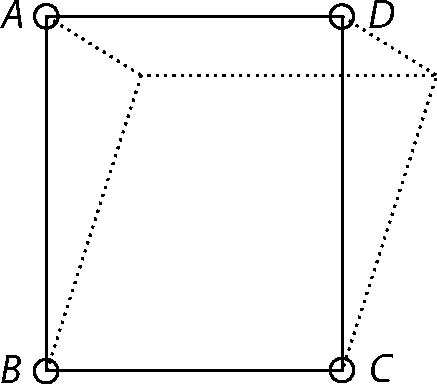
\includegraphics[width=0.280\textwidth]{gesamttex/edit_VIII-4/images/LH_38_04_184-d_184r.pdf}
\edcaption[0.75em]%
{%
\lbrack\textit{Fig.\:1}\rbrack%
}%
\end{edfigure}%
\newpage%
\vspace{3.0em}%
\pstart%
\noindent%
\centering%
*     *     *
\pend%
\vspace{4.0em}%
\selectlanguage{german}%
\frenchspacing%
\footnotesize%
\pstart%
\noindent%
\textls{Ausführliche Datierungsgründe:}%
\pagelabel{55813-E_dat}
Die titellose und undatierte Aufzeichnung N.\;\ref{55813-E} beschreibt schematisch eine Vorrichtung, die beim Aufbau eines tragbaren Barometers (\textit{aerometrum}) Anwendung finden sollte.
Dem Entwurf eines tragbaren Barometers widmet sich Leibniz insbesondere in den zwischen August und dem 12./22. November 1677 entstandenen, in diesem Band unter N.\;\ref{barom-portab_intro} edierten Aufzeichnungen.
Dies lässt die Vermutung zu, dass auch die Aufzeichnung N.\;\ref{55813-E} im Herbst 1677 entstand.
Eine frühere oder spätere Datierung der Aufzeichnung ist allerdings nicht auszuschließen.
Der Textträger weist weder Spuren eines Wasserzeichens noch weitere äußere datierungsrelevante Anhaltspunkte auf.
\pend%
\selectlanguage{latin}%
\frenchspacing%
\normalsize%
\newpage%
